\documentclass[a4paper,11pt, fleqn]{article}
%\usepackage[top=2cm, bottom=2cm]{geometry}

%\usepackage{color}
\usepackage[latin1]{inputenc}
\usepackage[T1]{fontenc}

%\usepackage[english]{babel} % is ja eigentlich alles auf englisch
\usepackage{graphicx}
\usepackage{listings}
\usepackage{floatflt, subcaption}

% set font to Palatino
\renewcommand*{\familydefault}{\rmdefault}
\renewcommand*\rmdefault{ppl}

\usepackage[backend=biber]{biblatex}
\addbibresource{bibliography.bib}
\usepackage[hidelinks]{hyperref}


\date{\today}
\author{Thats Me}

\begin{document}

\begin{titlepage}
		\raggedleft\textbf{\Huge Report Melodic Harmonization}\\
		\vspace{\fill}
		\centering Bla bla
\end{titlepage}
\tableofcontents 

% by Wolfgang
\section{Introduction} 
Artificial Intelligence (AI) is one of the most exciting topics in computer science; for research as well as for the public. We have seen impressive results of learning machines doing all kinds of difficult tasks. And there is general excitement among AI supporters about this technology and the future this might bring. 

Often these AI enthusiasts are criticized for there optimism in machines that can never act, decide and create on a human level, so the opinion of some critics. And in fact there are tasks that are beyond the capabilities of current AI approaches; where the goal is not clear and the direction of to the solution it is not visible. In this situations where the machine fails a human can often easily spot the right move to do and intuitively look for the answer in the right direction. This form of problem solving is based on creativity, a capability that is most often exclusively ascribed to humans. Another part of creativity that is not problem solving is inventing. This is the creation of innovative ideas and pieces. So what constitutes creativity and is it really exclusively present in biological machines that is the human? We think that in order to understand the human mind we have look at the things that make it unique. We also believe that creativity can artificially be reproduced and studied and can benefit the engineering and science. In this work we propose a method of procedural creativity and apply it to the music domain, by generating new music.

According to a popular theory of mind human cognition is nothing more than an information processing machine. A complex and very efficient machine though, but a machine. Following this idea we ask the question whether the possibility to implement aspects of creativity in an AI exists and what would be needed to do so. We have chosen the music domain for that. We implemented a program that is able to create new music after it has heard other music.

\subsection{The Music Domain}
We have chosen the music domain for several reasons. First it is an area that enables creativity, there is a whole culture around music creation and playing music. Even though creativity can be applied to any field (think about the creative problem solving) we wanted to work in a domain that is only 'solvable' with creativity, that way we at least have to approximate creativity mechanisms to get a result.

Secondly music has a representation on many different levels, similar to human cognition. On the basic layer sound are moving particles in a wave of high and low air pressure, that get interpreted as movements in the inner ear, similar there are pattern of firing neurons in the brain. If the air wave is constant we talk about tones. Music deals with tones on a scale. Starting at one root tone in music theory the tonality is built in a hierarchical fashion of intervals, i.e frequencies of the sound wave. At this layer of tone representation we normally start talking about music. It is clear that we already make some assumptions on how we perceive sound and what might sound good. Normally in western music we just consider the major keys, and we will do so in this work. Similar the brain builds concepts from raw firing pattern and uses them from more complicated operations.

The next layer are tones in the tonality ordered to a sequence. This layer describes what tones are played after another and what tones are played at the same time, in the music domain we normally talk of melody and harmony. We choose to work on this layer of symbolic representation. But there are even higher layers of music that are worth considering. There are different pieces of music and whole concerts with each a theme or a story and artists have different styles and genres. This higher levels of music make use of non music concepts such as stories and emotions. 

The interesting part about this is that all of these layers also are processed in a different way by humans. While creating (or just listening to) music all these layers are combined. But also the single layers are subject of inspection and one can be creative and inventive there as well. These properties are very useful for our exploration in computational creativity. This way we can focus on specific layers of the creative process and consider similar layers in the human cognition. By that we are able to build cognitive inspired models that can also be discussed on the basis of information processing in the human brain. 

\subsection{The Project Approach}
The main idea of the project is to build a computer program to test procedural creativity methods which are able to produce music on its own. 

To explore the methods we built a framework to test and explore computational accounts for music harmonization. This section will introduce this framework, later we will refer to the parts in more detail.

While designing the framework the guiding principles were molecularity and simplicity. The pipeline from input to output consisted of: Music representation - music piece (melody) - develop style - apply style to melody / harmonization - output music (e.g. musicxml)

Important to notice here is the differentiation between the 'creative' part and the harmonization part. We follow a two step process that consists of a style generation (creative) and the harmonization where this style is applied to the melody (deterministic). This way we can explore different 'creative' modules in our abstract representation and then have the same predictive harmonization process in the end, to project it back into music space.

\subsection{System Architecture}
The system's pipeline is visualized in Figure \ref{fig:arch}. The left side shows the input to the system, that consists of a melody to harmonize and a couple of known styles. All music that is input to the system is represented using our music representation using a sequence of vectors.
\begin{figure}
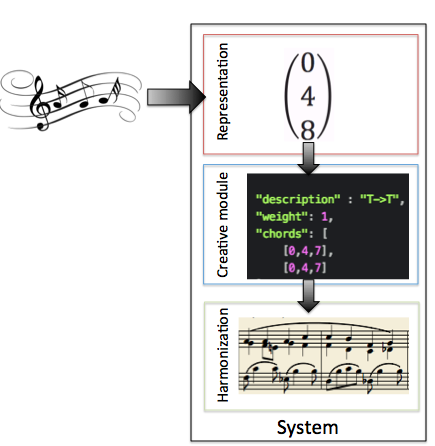
\includegraphics[scale=1]{Chapters/pic/sys_arch.png}
\caption{The architecture of the system}
\label{fig:arch}
\end{figure}


These styles are given by the user or generated out of other music or are the result of earlier runs and outcomes of the system.

The first part of the two step process is the creative part. Here the system creates a new style with given styles. This is where the creative algorithms are located. The user can choose one of the creative modules and different styles to create different new styles. In the next step the new style is then used as a template to harmonize the given melody. This step is not considered creative but made to be very predictive.

By splitting the process we are able to test different creative modules and produce just the style. We can then either just visualize the style as the essence of the creative module or run the deterministic harmonization process with a melody to be able to listen to the creation. 

\section{Implementation}


\section{Style}
Harmonic styles in the scope of this project are defined in terms of a name, a description and a list of weighted chord progressions (see Chords \& Progressions below). This is a strong simplification of the usual notion of a musical style, but thereby reduces complexity and allows formalization of an otherwise abstract concept.

Harmonic styles are implemented by the class HarmonicStyle, and specific manifestations are represented in terms of one JSON file (see JSON Format below) for each distinct style. With the help of static methods of the HarmonicStyleIO class, an instance of HarmonicStyle can be created from or serialized into a JSON file.

\subsection{Chord Progressions}
A chord progression is a list of two or more chords in fixed order. These chords are represented as a list of chromatic notes within one octave relative to an unknown reference note (e.g. the root of the melody's key). For example, the simple tonic could be expressed as (0,4,7). A perfect cadence could then be expressed as ((0,4,7), (2,7,11), (0,4,7)). The advantage of this relative definition is that it is independent of interpretation or musical function of specific notes and degree of the scale.

Actual chords can be obtained from these descriptions by defining a reference note, e.g. for the reference note C the former chord (0,4,7) would be equivalent to a chord formed by the notes C, E, G. Note that the given numbers do not indicate the octave or order of the given note. While the chord (2,7,11) stands for d, g, and b (for reference note c), the g could also be realized as the bass note. This is implemented as a normalization of the numbers into the range of (0,11), shifting all notes into the same octave. After normalization, the notes are stored as sets, i.e. each note can occur only once per chord.

Each chord progression in a harmonic style, characterized by its list of notes, additionally holds a weight. Its weight indicates how much it is preferred over other chord progressions, or specify the relative frequency of this progression in harmonizations developed from the harmonic style. These weights can be any number, but have to be consistent within the same harmonic style.

\subsection{JSON Format}
The JSON (short for: JavaScript Object Notation) http://tools.ietf.org/html/rfc7159 format is a light-weight, language-independent notation for data exchange, often used in client-server-applications. Data in the JSON format consists of attribute-value pairs and can therefore easily translated into associative arrays (e.g. dictionaries in Python). Utilization of this format has many advantages: It is human-readable and is used by many computer programs and web-applications. Therefore, by using the JSON format, we can make use of the libraries and interfaces programming languages and other software (e.g. Music21) provides. An example of a chord progression defined in JSON format can be seen in Fig. X.

\begin{verbatim}
{
	"description" : "T->T",
           "weight": 1,
           "chords": [
                [0,4,7],
                [0,4,7]
           ]
}
\end{verbatim}

\subsection{Creativity}

The creativity module is used to develop a new harmonic style from a given harmonic style in a possibly creative way.
While the input and output are always both style descriptions, each implementation of this module can have additional parameters that influence the derivation of the new style from the old one.
There are currently two implementations of this module, one that is completely random (\texttt{RandomCreativity}) and one that is a very simple collection of ideas that are related to creativity (\texttt{SimpleCreativity}).

An implementation of the creativity module is a class that implements the method \texttt{develop}.
This method takes as inputs a \texttt{HarmonicStyle} and two strings for the name and the description text of the output style.
It then returns a new \texttt{HarmonicStyle}.
Additional parameters can be given via the constructor of the class.

\subsubsection{RandomCreativity}

\texttt{RandomCreativity} takes two parameters in the constructor:
A standard deviation factor $f_\sigma$ and a flip chance $p$.
It takes the chords and progressions from the input style and randomizes them according to two rules:
The weight of each progression is updated randomly according to a normal distribution
\[ w' \sim N(w, (w f_\sigma)^2)\]
where $f_\sigma$ is the given standard deviation factor.
Each chord in each progression is changed randomly flipping its notes where flipping means adding the note to the chord if it did not belong to the chord before or removing it from the chord if it did.
For each possible note (0-11) a Bernoulli trial where the success probability is the flip chance $p$ is used to determine whether the note should be flipped.
This implementation of the creativity module is just used as a dummy.

\subsubsection{SimpleCreativity}

\texttt{SimpleCreativity} tries to combine some general considerations about creativity with random variation.
Intuitively, there are at least two requirements for calling something creative:
It must be \emph{new} and in some sense \emph{good}.
The first requirement seems to the more obvious one:
Something that is just a copy of something that already existed before is not creative.
While it can be (and probably in most cases is) based on something existing it must be different at least in some respect.
In our case, it is relatively straightforward to find measures for the similarity or dissimilarity of chords or chord progressions, as they are very structured.
For example, since a chord can be seen as a mapping from a pitch class (0-11) to a truth value (where true means that the chord contains the pitch and false that it does not), two chords can be compared by the places in which they differ.

The second requirement might seem a bit surprising in the light of things like contemporary music and art, which might seem very unpleasant or ugly to some.
But it is important that even in those cases there can be some kind of quality measure in the sense that there is a justification of the outcome and that it is not arbitrary.
Even for a work in which randomness is used there is usually an idea behind it.
For example, a piece of music that, as a result of bad composing, has awkward harmonic progressions and a strange melody is probably not very creative.
On the other hand, a piece that is based on a complicated algorithm that determines its notes and that has been chosen for a very specific reason might be considered very creative although it does not sound very nice.

The difficulty lies in the quality measure itself, which is not fixed and usually not given beforehand.
Therefore, we are in a dilemma between fixing a quality measure for our task, which might prohibit some outcomes that would be considered creative according to different quality criteria, and not fixing it, which basically leaves the task underspecified.
We do not want to restrict creativity to things that sound pleasant, but we also want to distinguish between good and bad compositions.

As a solution, one might go with mathematical and physical properties of the music itself and psychoacoustic phenomena that are shared by humans as guidelines for a very general but rigid quality measure for the harmonic styles we have in mind.
This is not the only possible solution since it prohibits certain types of creative music like the algorithmic composition in the example above, but it is practical if our goal is to find music that does not just copy what already exists but still sounds pleasant.

The class \texttt{SimpleCreativity} is a first and very rough attempt to follow this idea.
It splits the development of the new harmonic style into two phases: a generation phase and a selection phase.
In the generation phase new musical material is generated in the form of fragments of chord progressions (i.e., chord progressions that contain few chords or even only a single chord).
The selection phase tries to select the ``good'' material and to combine it to larger progressions according to some heuristics.

The generation phase uses the same techniques as the \texttt{RandomCreativity} to generate new chords from the ones in the input style.
Furthermore, it takes the given chord progressions and splits them randomly into smaller parts.
This allows the existing progressions to be recombined in novel ways in the selection phase.

The selection phase uses substition and concatenation to create new progressions from the existing progressions and the newly generated ideas.
Substitution candidates are found by comparing the all new chords (i.e., those that are contained in the new ideas but not in the original style) to the old chords according to the similarity measure described above scaled to 1 (i.e., divided by 12).
A threshold for the similarity of substitution pairs can be given to the constructor of \texttt{SimpleCreativity}.
If the old chord of a substitution pair is found in one of the old progressions, the ``plausibility'' of substituting it with the new chord of the pair in that context is calculated based on the relation between the new chord and its neighbours in the progression.
The relevant properties are the similarity of the latter chord to the falling fifth of the former chord and the stepwise movement of notes from one chord to another.
If the plausibility is high enough (again, a threshold can be given via the constructor), the substitution is performed.

Concatenation of fragments to larger progressions is currently not implemented.
In the harmonization process, progressions are concatenated anyways, so the only reason to do this already at this point would be to give a certain combination a higher weight than the sum of the weight of its parts in order to prefer it to other possible combinations.
However, we did not find a plausible criterion for when this should happen.

\subsubsection{Further Ideas}

It is questionable whether the distinction between generation and selection phase is a good idea.
One could also think of a setting in which there is a feedback between both phases.
Also, harmonic structure is usually not developed in isolation but in relation to other musical parameters depending on specific situations.
Therefore it might be required to incorporate models of other musical parameters into the process.

The generation phase is currently random and unbiased except for the structure of the input and output and the specific randomization method (i.e., what exactly is randomized and what not).
A different possibility would be to already include heuristics with respect to the musical content of the ideas, i.e. to only generate ``good'' or at least promising ideas according to some quality measure.
Also, the structure of the output of this phase as (possibly partial) chord progressions could be extended to allow other types of ``ideas'' that are, for example, parametric.

The selection phase could be adapted to a more sophisticated and more general psychoacoustic model than the current ``falling-fifth-plus-stepwise-movement'' approach.
Another possibility would be to put the generated ideas into a more general musical context, e.g., to generate melodies, harmonize them using different selection candidates and thus measuring the quality of the selection candidates.
These two approaches could also be combined by applying the psychoacoustic model not to selection candidates but to the harmonizations generated from them.


\subsection{Harmonizer}
The harmonizer is responsible for finding the ``best'' harmonization, with respect to the weights of each progression defined in the harmonic style, for a given melody. It is defined in the Harmonization class and treats all possible sequences of chord progressions and their weights as a shortest path graph problem. Therefore it makes use of the NetworkX library,\footnote{https://networkx.github.io} a popular python library providing classes and algorithms for working with networks and graphs. 

The algorithm of the harmonizer can be summarized by the following steps:
\begin{enumerate}
  \item Find all potential progressions
  \item Build a graph from these progressions
  \item Find the shortest path in the graph
  \item Build a list of progressions from the shortest path
\end{enumerate}
These steps are depicted further in the following paragraphs, figure \ref{fig:4} shows the harmonization process of the melody ``0, 0, 0'' with the harmonic style defined in ``dummy\_style.json''.

\subsubsection{Finding Potential Progressions}
The harmonization algorithm starts with an harmonic style (as defined above) and a melody as input. Furthermore, the keynote and octave are given by the user in order to ``ground'' the output of final harmonization to specific notes instead of relative intervals. The maximum weight of all potential progressions is saved in order to normalize all weights later on, in order to find the shortest path (i.e. smallest sum of weights) instead of the longest.

For each note in the melody, all progressions in the harmonic style are iterated and each progression is checked whether it is a potential harmonization for the considered note. This is the case if the length of the progression is shorter than the length of the melody after the considered note (i.e. the progression is not longer than the remaining melody) and the considered and following notes are included in the respective chords of the progression. If this holds true, the progression is saved as a potential harmonization for the considered and the following notes.

\subsubsection{Building the Graph}
From these potential progressions, a directed weighted graph is built to be able to perform a path search with established graph search algorithms. First of all, a ``START'' node is added to the empty graph. For each potential progression for the first note of the melody, a node is created annotated with the first chord of the progression and a ``1'' indicating the current position. The position is attached to the node to account for progressions of different lengths. This set of nodes is then connected to the starting node. (Fig. \ref{fig:41})

Additionally, a node is created for every last chord of the progressions, again annotated with the chord and position (depending on the length of the progression). An edge is added between two nodes if the transition is possible, indicating the chord progression itself and the weight taken from the harmonic style. (Fig. \ref{fig:42}) All weights are calculated by subtracting the actual weight from the maximum weight, therefore the largest weight gets weight 0 and we have to solve a shortest / cheapest path problem, for which more algorithms exist. If more than one transition between two nodes is possible, only the progression with the largest weight is considered since all others can not be part of the best path.

This procedure is repeated until the nodes for the potential harmonization of the last note of the melody are created. These are then connected to the ``END'' node, and a path can be searched for between ``START'' and ``END'' node. (Fig. \ref{fig:43})


\subsubsection{Shortest Path}
As described above, the progressions with the largest weights in the style definition (= most desirable progressions) possess the smalles weights in the graph. Therefore the algorithm has to find the shortest path (weights are seen as distances) between the ``START'' and ``END'' nodes. We decided on the Dijkstra algorithm for this matter, since we are looking for a single source path in a graph with non-negative weights. To speed up computation for long melodies or extensive harmonic styles, we used a bidirectional implementation. The path found by this algorithm in the example graph can be seen in Fig. \ref{fig:44}.

% bidirectional dijkstra https://en.wikipedia.org/wiki/Dijkstra's_algorithm https://en.wikipedia.org/wiki/Bidirectional_search
% figure of dijkstra
% optimization problem

\subsubsection{Final Harmonization}
In the final step, the algorithm creates the list of chords representing the final harmonization. This is achieved by iterating the nodes of the shortest path from starting to final node, appending the chords attached to the edges connecting the nodes. This list of chords is then returned to the calling function and can further be worked with.

\begin{figure}[!tbp]
\vspace*{-3cm}
\centering
\begin{subfigure}[b]{0.43\linewidth}
   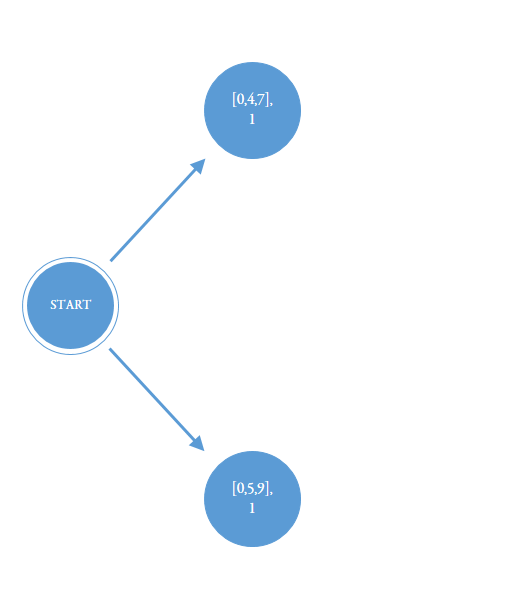
\includegraphics[width=\linewidth]{Chapters/pic/41}
   \caption{Adding START node and first chords of first progression}
   \label{fig:41} 
\end{subfigure}
\hfill
\begin{subfigure}[b]{0.49\linewidth}
   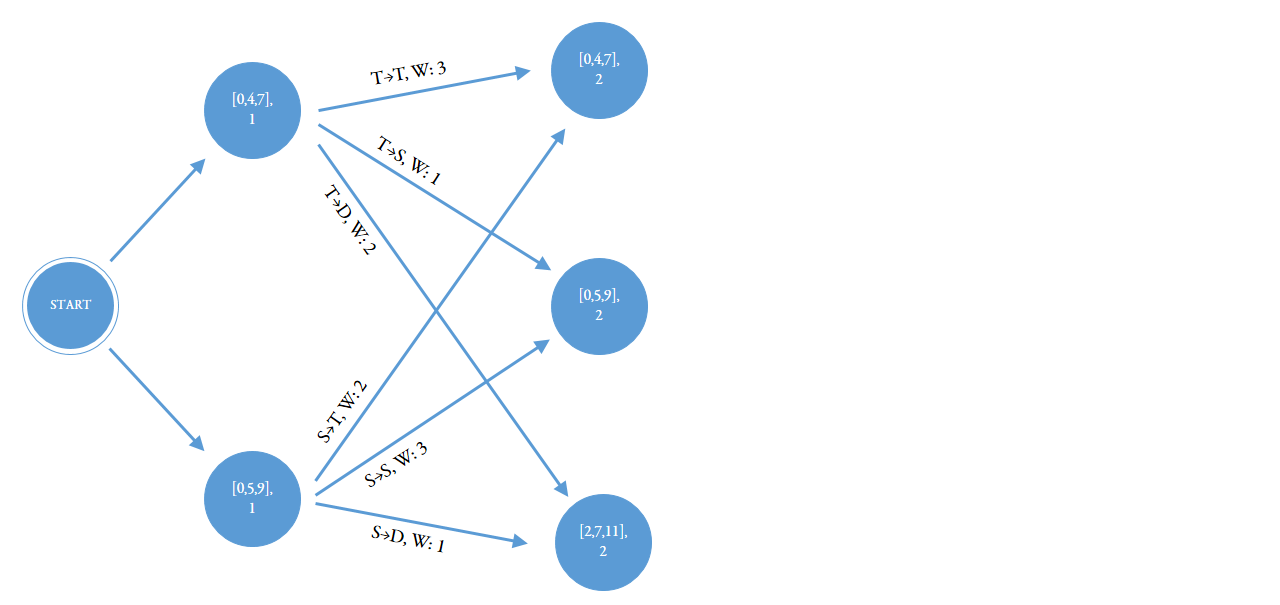
\includegraphics[width=\linewidth]{Chapters/pic/42}
   \caption{Adding last chords of first progression}
   \label{fig:42}
\end{subfigure}

\begin{subfigure}[b]{1.2\linewidth}
   \hspace{-1.1cm}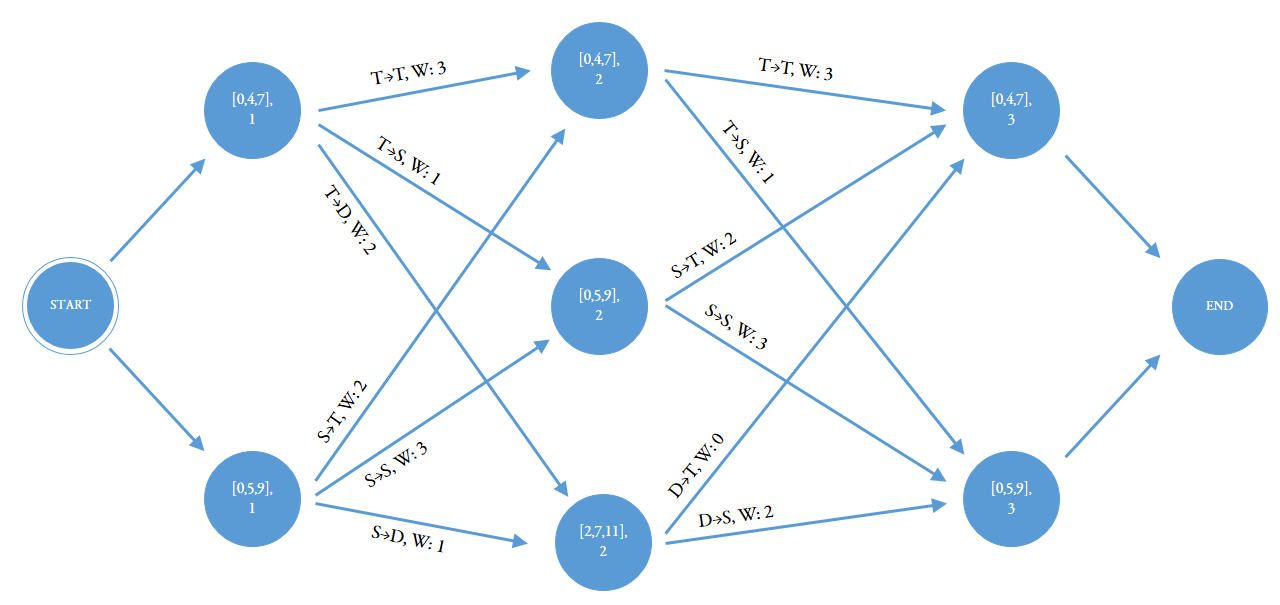
\includegraphics[width=\linewidth]{Chapters/pic/43}
   \hspace{-1.1cm}\caption{Completed graph for melody ``0, 0, 0''}
   \label{fig:43}
\end{subfigure}

\begin{subfigure}[b]{1.2\linewidth}
   \hspace{-1.1cm}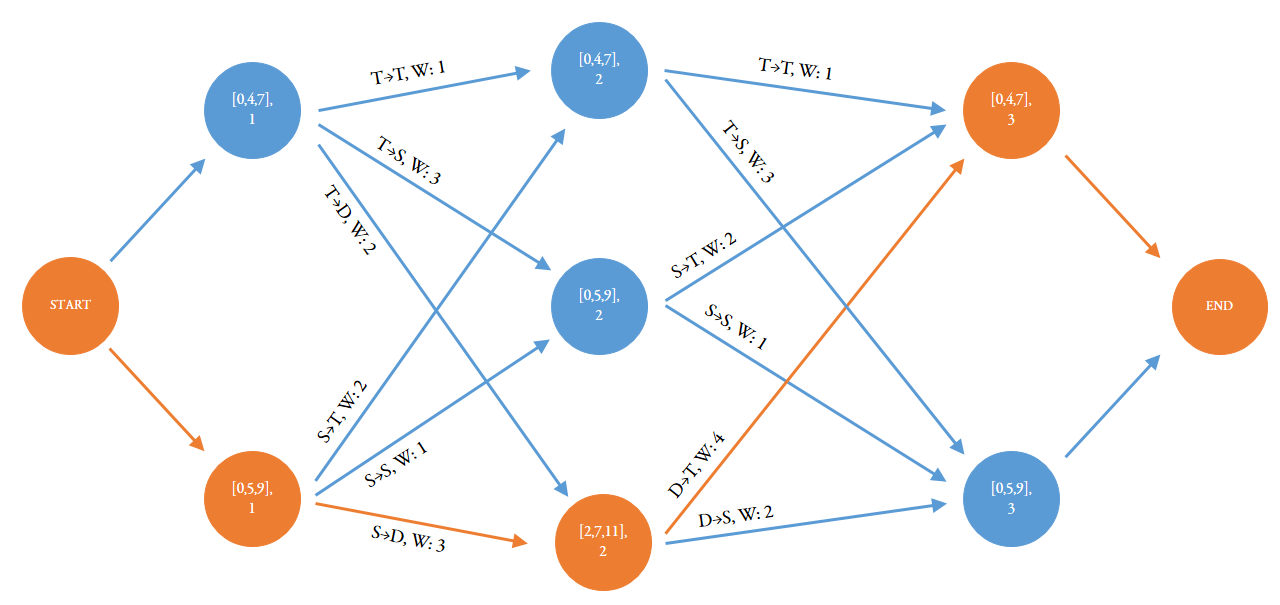
\includegraphics[width=\linewidth]{Chapters/pic/44}
   \hspace{-1.1cm}\caption{Shortest path found by bidirectional Dijkstra}
   \label{fig:44}
\end{subfigure}

\caption{Selected steps of the harmonization with ``dummy\_style.json''}
\label{fig:4}
\end{figure}



% TBD by Wolfgang
\section{Style Viewers} 
As we have shown earlier, the style views are the essence of the creative process so it's worth looking at this in its' raw form. That's why we included some style viewer in to project to apply to this task. In this section we introduce them.

\subsection{Text Based viewer}
As discussed earlier the styles are saved in a JSON file. Also these are made to intellectual by humans we thought of a more pleasant way to view the style wile developing. So we gave the style objects a print method. This method will print the style onto the current output of your python session. As seen in the figure below:

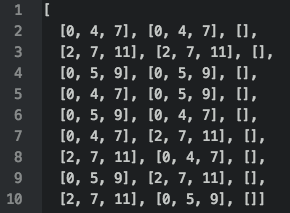
\includegraphics[scale=1]{Chapters/pic/text_print.png}

This figure shows the dummy style. The viewers orders the all the style sequences according to there likelihood, starting with the most likely.  It also translates our numeric representation into a tonal representation for a given key (default key is C major).

That way one can easy see what the style will look like and if after applying the creative module, odd thing happened to the style, that would be harder to spot after the actual harmonizer. 

\subsection{MusicXML Creator}
Also fast and more visual would be to translate the style into a musicXML file and view it with your favorite musicXML viewer. We used MuseScore for that purpose. 

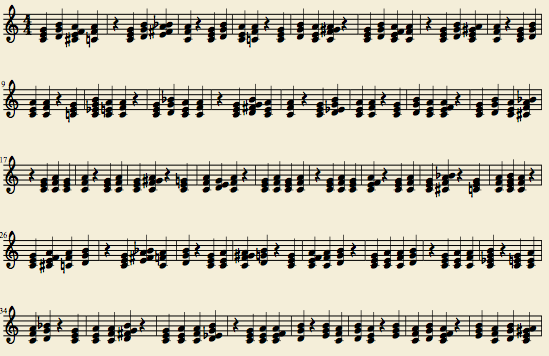
\includegraphics[scale=.5]{Chapters/pic/xml_print.png}

As seen in figure above we did it for the dummy style. To do that we used the $write_musicxml$ method of the visualizer. It dose the same thing as the print method, that it orders the chore sequences starting with the most likely. But instead of printing it to the output it creates the musicxml file. For convince we defined a bunch of default values., that are: key is C major, duration if a tone is quarter pitch, as well as we use a four quarters rhythm. After every sequence we inserted a quarter break to indicate the end of a harmonization sequence.

With this visualization you have the major advantage that now you have standardized data structure and you are able to process them farther. But mainly you want to show it in a score notation or listen to your creation.

This is where this ends, because now we have a wildly compatible format that can be used in to do any more complicated things you may want to do. 

\section{Related Work}

\subsection{Additional Tools}
\label{sec:tools}

Here, we will list some additional tools that were used in the context of this project.

\subsubsection{Extempore}
\label{sec:tools.extempore}

Extempore \cite{extempore} is a programming environment for live coding.
It features a scheme interpreter and a just-in-time compiler for its own language xtlang, a low-level language with a Lisp syntax.
Scheme is usually used for application logic such as algorithmic composition or application control while xtlang allows to program the synthesis of sound, displaying of graphics, or other computations with real-time requirements.

Sound is created by defining the \texttt{dsp} function which takes inputs like a time code, an input sample, and a channel and returns an output sample.
The way in which the output sample is generated is left to the programmer and can include, for example, synthesis or sampling.
Extempore's standard library provides help for the sound generation on the sample level as well as composition on the note level (scales, chords, etc.).
One core idea of Extempore is the concept of temporal recursion: a function can schedule another call to itself at a later point in time creating a loop with exact timing that can be modified on the fly.

In the context of this project, Extempore is used for making a style audible as described in Section \ref{sec:viewers.extempore}.

\subsubsection{Music21}
\label{sec:tools.music21}

Music21 \cite{music21} is a Python library for the computational analysis of music.
It includes a set of annotated corpora and analysis tools as well as general music theoretical utilities.
Data from the corpora can be accessed as Python objects and transformed, manipulated, and analyzed in Python.
The example style \texttt{coltrane.json} has been generated using Music21.

\subsubsection{Lilypond}
\label{sec:tools.lilypond}

\textit{Is this used at all?}

\subsubsection{Musescore}

MuseScore \cite{musescore} is an open source music sheet editor.
It can display and play sheet music and supports MusicXML and Lilypond formats.
This project uses it to view and listen to MusicXML representations of styles.
Another idea was to make the harmonizer available as a plugin in MuseScore.

\subsection{Related Research}

\subsubsection{Rohrmeier}

\subsubsection{Koops - \textsc{HarmTrace}}
The work by \cite{koops2012} is a model based system to derive harmonic functions of chords in their tonal context and consists of \textsc{HarmTrace} and the \textsc{HarmTrace Harmonizer}. It is a rule based system written in the programming language Haskell. Given a chord sequence \textsc{HarmTrace} derives the harmonic function of the of a chord in it's tonal context. It describes a grammar to represent chords and the relations between them in them. Based on this representation the \textsc{Harmonizer} creates the best fitting chord sequence to harmonize the melody.

The system involves three steps. First the melody is analyzed using the \textsc{HarmTrace} program. After that the tonality and the and the time signature of the music piece is represented in a data structure that defines a context free grammar. After that the best sequences of chords are selected using the \textsc{HarmTrace Harmonizer}. 

This selection is based on basic heuristics form the harmonization theory, like the circle of fifths and cadences. The system includes four steps: Generating, Selection, Parsing and Post-processing. 

\paragraph{Generating} 
The system takes as single track as input and extracts tonality and rhythm information of the piece using the \textsc{HarmTrace} module and represents it in the context free grammar. In this representation the possible chords are calculated for the root note and a pre-selection is done. Next the probabilities are assigned to the chords in the remaining set, which are calculated using the circle of fifths, where the distance of the melody note to the root note gives the probability. The circle of fifths is used because it corresponds with human perception of harmony. 

\paragraph{Selecting sequences}
In the next step the probabilities are used to generate a list of possible harmonization chord sequences. The list is generated by randomly selecting from the chord candidates. The probability distribution for that is defined by the chord probabilities, calculated before. 

\paragraph{Parsing}
In this step the short chord sequences are combined to a lager piece using the \textsc{HarmTrace} parsing capabilities, so that the best sequence of chords progressions if returned. The best sequence is determined by the best fit with the grammar.

\paragraph{Post-processing}
In the final step the symbolic representation of the music piece is translated in the MIDI format. For that some heuristics are used to ensure that the resulting piece will sound good. 

\paragraph{Relation to our work}
This work is related to our project it the sense that is also uses a symbolic representation of music and creates harmonization of the piece automatically. Similar to our work Koops uses representations to generate new chords and sequences. He also represents the chords in therms of relive distance between the tone and the root similar to our representation.

Other then in our work he uses a pre-selection step to exclude chord sequences from the pool if generated chords. This is done by using the concept of cadences and the circle of fifths. That way he wants to ensure that the result is not bad by chance. We instead regularize the output by giving the system only the limited number of sequences to work with, that are the styles we put in the system at the start. 

Koops also uses the circle of fifths in combination with a stochastic selection to generate new sequences, this is a good idea to ensure that the result will sound good. The disadvantage of this approach is that the result wouldn't sound interesting because it favors the close and common chords. Because of this random generation paired with a strong heuristics selection the system is not inventive enough for us to grant creativity to it.





  

\section{Outlook}

\subsection{Applications}

\subsection{Limitations}



\noindent
Todo:\\
- References nach Biblatex\\
- Music21\\
- Applications\\
- Limitations\\
- Creativity\\
- Related Work (Koops, Rohrmeier, Bobs Kram)

%% TBD by Wolfgang
%acctually last chapter ?? Ch9
\section{Related Work} 
In this section we introduce the Koop's Paper and campare the approach to our ideas...TBD

\printbibliography

\end{document}